\documentclass[12pt,a4paper]{article}


\usepackage{graphicx}
\usepackage{amsmath, amsthm, amssymb}
\usepackage[english]{babel}
\usepackage{epstopdf}
\usepackage{geometry}
\geometry{a4paper,top=2.5 cm,bottom=2 cm,left=2.5 cm, right= 2.5 cm}


\title{The liquid-solid transition
	\\{\small{Statistical Mechanics}}
\author{\small{Daniele Scarinci}}}


\begin{document} 
\maketitle
\abstract{This report deals with the liquid-solid transition, analyzed trough the use of mean-field theory. The first part will introduce the basic concepts of mean-field theory while the second will focus on studying the liquid-solid transition}

\tableofcontents

\section {Mean-field theory}

Mean-field theory is an approximation for the thermodynamics properties of a system based on treating the order parameter as spatially constant. It's an useful description if spatial fluctuations are not relevant, and it becomes an exact theory only when the range of interactions becomes infinite. It's very useful, since it makes quantitatively correct predictions about some aspects of phase transitions in high spatial dimensions where each particle or spin has many nearest neighbors, and it is also relevant in physical dimensions. Mean-field theory has also the enormous advantage of being mathematically simple.
At high temperatures, since there is no order, the order parameter $\langle \phi \rangle$ is zero. At a critical temperature $T_c$, order starts to appear and $\langle \phi \rangle$ becomes different from zero. If $\langle \phi \rangle$ rises continuously from zero, the transition is a second order one, while if $\langle \phi \rangle$ jumps discontinuously to a value the transition is called a first order transition. The heat adsorbed in a first-order transition switching phase is called the latent heat $Q_L=T_c \Delta S$, where $ \Delta S$ is the entropy change and $T_c$ is the transition temperature.
There are many formulations of mean-field theory, such as the van der Waals equation of state for the liquid-gas transition, the Weiss molecular field theory for ferromagnetism and the Bragg-Williams theory. The last one leads to Landau phenomenological mean-field theory, which is based on a power series expansion of the free energy in terms of the order parameters for the transition of interest. This assumes that the order parameter $\langle \phi \rangle$ is "small" so that only the lowest order terms required by symmetry are kept. In situations in which order parameters are not small, more complete mean-field theories such as Bragg-Williams theory, are chosen.

 \section{The liquid-solid transition}

\subsection{Introduction}

 In the liquid phase, the average density $\langle n(\textbf{x}) \rangle$ is spatially uniform, while in the solid form it's a periodic Fourier series expansion in terms of reciprocal lattice vectors $\textbf{G}$:
\begin{equation} \label{inizio}
\langle \delta n(\textbf{x}) \rangle = \langle n(\textbf{x}) \rangle - n_0 =\sum_\textbf{G} n_\textbf{G} e^{i\textbf{G} \cdot \textbf{x}}
\end{equation}
with $n_0$ as the average uniform density, the vectors $\textbf{G}$ in some reciprocal lattice and, since $\langle \delta n(\textbf{x}) \rangle$ is real, $ n^*_\textbf{G} = n_\textbf{G}$. We can say that the order distinguishing the liquid phase from the solid one is one of spatial modulations. As is known, the statistic structure function $S_{nn}(k)$ for a liquid has a maximum on a sphere of radius $k_0 = 2 \pi / l$ (where $l$ is the average interatomic separation). As the temperature is lowered, the magnitude $S_{nn}(k_0)$ increases, and it's therefore reasonable, to describe the liquid-solid transition, to consider only the maximum peak and approximate $S_{nn}(k)$ in the vicinity of $k=k_0$ by
\begin{equation}
\label{eq:kappa}
S_{nn}(k)=\frac{T}{[r+c(k^2-k^2_0)^2]}
\end{equation}
 where $r=a(T-T^*)$ decreases with $T$, leading to an increase in $S_{nn}(k)$, and $S_{nn}(k)$ is the Fourier transform of the density-density correlation function
\begin{equation}
S_{nn}( \textbf{x}, \textbf{x} ^\prime)= \langle \delta n(\textbf{x})\delta n(\textbf{x}^\prime) \rangle
\end{equation}
The temperature $T^*$, which is in general a function of $n_0$, will turn out to be the mean-field limit of stability of the liquid phase.
Now, since $\chi( \textbf{x} ,\textbf{x} ^\prime) = T S_{nn} ( \textbf{x} ,\textbf{x} ^\prime)$ is the derivative of the free energy  with respect to $ \langle \delta n(\textbf{x})\rangle$ and  $\langle \delta n(\textbf{x}^\prime)\rangle$, an equation for the free energy which predicts Eq.(\ref{eq:kappa}) for $S_{nn}(k)$ in mean-field theory is simply:
\begin{equation} \label{eqbau}
F_{SL} = \int d^d x d^d x^\prime  \langle \delta n(\textbf{x})\rangle \chi^{-1}_{0}( \textbf{x} ,\textbf{x} ^\prime) \langle \delta n(\textbf{x}^\prime)\rangle - w \int d^d x \langle \delta n(\textbf{x})\rangle ^3 + u \int d^d x \langle \delta n(\textbf{x})\rangle ^4
\end{equation}
 where
\begin{equation}
\chi^{-1}_{0}( \textbf{x} ,\textbf{x} ^\prime) = [ \textbf{r} + c(\Delta ^2 + k^2_0)^2] \delta(\textbf{x} - \textbf{x} ^\prime)
\end{equation}
We assumed that in Eq.(\ref{eqbau}) $\langle \delta n(\textbf{x})\rangle$ has Fourier components in the vicinity of $|\textbf{k}| = k_0$, which means that the wave vectors near the origin are explicitly excluded. It shoud also be said that $k_0$ is the only true parameter in the theory, while $w$, $u$, $c$ and $T^*$ can depend on other parameters such as density or pressure (as we will see later on). 

Using the Fourier decomposition of Eq.(\ref{inizio}), we get that
\begin{equation}
\begin{split}
&f_{SL} = \frac{F_{SL}}{V} = \sum_{G} \frac{1}{2}r_{G}|n_{G}|^2 + \\ &- w\sum_{G_1,G_2,G_3} n_{G_1}n_{G_2}n_{G_3}\delta_{G_1+G_2+G_3,0}+\\&+ u\sum_{G_1,G_2,G_3,G_4} n_{G_1}n_{G_2}n_{G_3}n_{G_4}\delta_{G_1+G_2+G_3+G_4,0}
\end{split}
\end{equation}
where $r_{G} = r + c(G^2 - k^2_0)^2$.
\newline
Thus, since there is a third order term in the free energy, this will lead to a first-order transition. The solid phase is far more complicated than the liquid one, and to specify it completely we need all of the infinite vectors $\textbf{G}$ in the reciprocal lattice. So, to discuss the liquid-solid transition, we need a minimization of $f$ with respect to $n_{\textbf{G}}$ for all the possibles lattice candidates. The set of $n_{\textbf{G}}$'s that give the lowest value of $f$ determines the equilibrium configuration. For this reason very few thing can be said in general about the liquid-solid transition, however, the fact that only certain lattices have reciprocal lattice vectors that add to zero in triangles, allows to make some general statements about this transition when it is only weakly of the first order.
\subsection{Are all crystals BCC?}
We will now simplify the problem by allowing c to go to infinity, obtaining that all wave vectors $\textbf{G}$ will have magnitude $G=k_0$, allowing us to consider only vectors that lie on a sphere in reciprocal space. The third-order term we discussed above favors lattices whit triads of vectors that add to zero and in our case this will be possible only if the $\textbf{G}$'s form an equilateral triangle. There are only different sets $L_G$ of equal length vectors containing closed triangles, $\textbf{G}$ and $-\textbf{G}$ that form symmetric structures (shown in the figure below):
\begin{itemize}
\item The set of six edge vectors of an equilateral triangle and its inverted image (a)
\item The set of 12 edge vectors of an octahedron (b)
\item The set of 30 edge vectors of an icosahedron
\end{itemize}
\begin{figure}[h!]
\begin{center}
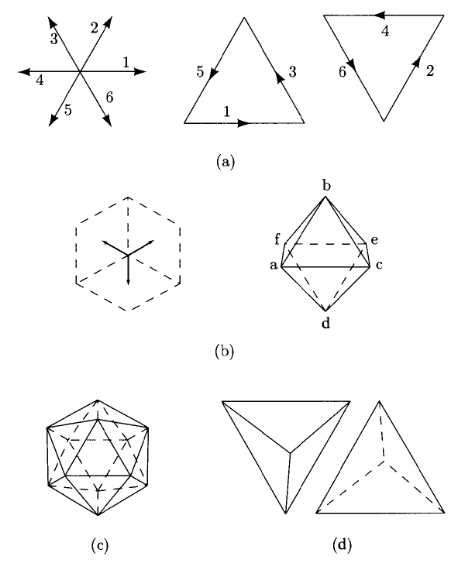
\includegraphics[width=10cm]{robi.png}
\end{center}
\caption{(a) Six shortest vectors in a hexagonal reciprocal lattice and the two independent triangles that can be formed from these vectors. (b) Shortest vectors of the FCC reciprocal lattice: the figure on the left shows one octant of the FCC reciprocal lattice with three of the 12 shortest vectors, and the figure on the right shows the 12 shortest vectors arranged on the edges of an octahedron. The square acef in the octahedron is planar, and the diamond abcd is non-planar. (c) An icosahedron. (d) A tetrahedron and its inverted image.}
\label{fig:robi}
\end{figure}
The three cases correspond to planar hexagonal, FCC and icosahedral reciprocal lattices. The FCC lattice with lattice vectors $\textbf{G} = 2^{-1/2}G (\pm1,\pm1,0),(\pm1,0,\pm1),(0,\pm1,\pm1)$ corresponds to a BCC direct lattice. The case (d) in the figure above was not included since that set is identical to that of the octahedral edges.

In order to calculate $f$, we need to evaluate $f_2, f_3$ and $f_4$, that is, the terms of $f$ of second, third and fourth order in $n_G$. The second-order term is proportional to the number of vectors $m$ in $L_G$, and we therefore choose $n_\textbf{G} = m^{-1/2}n_G$ for every $\textbf{G}$. In this way we have assured that $f_2 = \frac{1}{2} r n^2_{G}$ has the same form for every lattice. $f_3$ depends on the number of triangles $p$ to which each vector belongs. and is equal to one for the hexagonal and is equal to two for the FCC and icosahedral lattices. We can evaluate $f_3$ stating that in $n_{\textbf{G}_1}n_{\textbf{G}_2}n_{\textbf{G}_3}$ there are $m$ choices for $\textbf{G}_1$. Once we choose $\textbf{G}_1$, there are $2p$ choices for $\textbf{G}_2$ (there are two free edges in each of the $p$ triangles to which $\textbf{G}_1$ belongs). We then have only one choice for $\textbf{G}_3$. Thus, we have that:
\begin{equation}
f_3=-2wpm^{-1/2}n^3_G
\end{equation}
The evaluation of $f_4$ is more complicated, but we finally get that our final result for $f$ will be:
\begin{equation}
f=\frac{1}{2}rn^2_G-2wpm^{-1/2}n^3_G+6u(1+\frac{q}{m})n^4_{G}
\end{equation}
From this equation we can see that the favored phase will be the one with the biggest value of $f_3$ compared to $f_4$. The fourth term in fact does not change the preferred lattice, but it's actually important in determining the actual transition temperatures. Calculating the transition temperature using the first-order isotropic-to-nematic transition analysis, we obtain:
\begin{equation}
\begin{split}
r_c=a(T_c-T^*)=\frac{1}{2}\frac{(2wp)^2}{6u(m+q)}=\\
=\frac{w^2}{3u}\begin{cases}\frac{1}{6}\text{\:\:\:\:hex\:\:\:\:} m=6, p=1, q=0 \\
\frac{1}{4}\text{\:\:\:\:BCC\:\:\:\:} m=12, p=2, q=4 \\
\frac{2}{17}\text{\:\:\:\:icos\:\:\:\:} m=30, p=2, q=4 
\end{cases}
\end{split}
\end{equation}
As we expected, the transition temperature $T_{BCC}$ to the BCC phase is the highest, and further analysis shows that the BCC lattice is the stable one of the set, considering $T<T_{BCC}$. If we needed to treat realistically the possible formation of the other lattices, like FCC, we would have need to include higher order terms in $n_{\textbf{G}}$ and not to neglect the secondary peaks in $S_{nn}(k)$.

In nature a large number of materials crystallize from the melt into BCC. For example, all metallic elements on the left hand side of the periodic table, with the exception of Mg and almost all of the lanthanides and actinides, from BCC structures near the melting point.

\subsection{Criterion for freezing}
$S_{nn}(k)$ evaluated at the maximum of its first peak at $|\textbf{k}|=k_0$ reaches a maximum value of $T_c/[a(T_c-T^*)]$ at the liquid-solid transition. Trying to evaluate the ratio between $S_{nn}(K_0)$ and $S_{nn}(\textbf{k}=\infty)=n_0$ using molecular dynamics calculations on gases of particles interacting via a Lennard-Jones potential or via a Coulomb interaction, predicts a value of order 2.7 at $T_c$. This is called the \textit{Hansen-Verlet criterion}. Experiments on many systems tend to confirm this result. As a liquid is cooled, the first peak grows and, as $S_{nn}(k_0)/n_0$ becomes bigger than 2.7, solidification usually occurs. To get a quantitative prediction of this ratio from mean-field theory we will have to specify the values of the phenomenological parameters $a$, $w$ and $u$. The $w$ parameter has the units of $E\cdot V^2$ and $u$ is $E \cdot V^3$, so that $w^2/u$ has units of energy times volume. Since the natural units of energy and volume in our problem should be $T_c$ and $n^{-1}_0$, we will write $w^2/u=bT_cn^{-1}_0$, where $b$ is a numerical factor of order one. Thus we will have that $S_{nn}(k_0)/n_0=T_c/(2w^2n_0/21u)=21/2b$, and the phenomenological Verlet criterion can be satisfied with $b=4$.

\subsection{Improvements of the theory}
In nature we don't observe only BCC structures, so, how is this possible? In the theory we presented we made a major approximation stating that $|\textbf{G}|=k_0$, obtained by setting $c=\infty$ and ignoring higher order peaks in the liquid structure factor. If this restriction is lifted, then the third-order term will couple $n_{\textbf{G}}$ with $|\textbf{G}|=k_0$ to $n_{\textbf{G}_2}$, with $|\textbf{G}_2|\neq k_0$. We will have contributions $f$ of the form:
\begin{equation}
f^\prime_2=\frac{1}{2}m_2 r_{\textbf{G}_2}|n_{\textbf{G}_2}|^2-vgn_{\textbf{G}_2}^2n_{\textbf{G}_2}
\end{equation}
where $m_2$ is the number of wave vectors $\textbf{G}_2$ equal to the sum of two vectors $\textbf{G}$ of magnitude $k_0$, and $g$ is a combinatorial factor. Minimizing $f^\prime_2$ with respect to  $n_{\textbf{G}_2}$, we find:
\begin{equation}
n_{\textbf{G}_2}=\frac{vg}{m_2 r_{\textbf{G}_2}}|n_{\textbf{G}_2}|^2
\end{equation}
and
\begin{equation}
f^\prime_2=-\frac{1}{2}\frac{v^2g^2}{m_2r_{\textbf{G}_2}}|n_{\textbf{G}_2}|^4
\end{equation}
leading to a negative correction to the coefficient $u$ in the total free energy. If only the first ring in $S_{nn}(k)$ is kept but the condition $c=\infty$ is relaxed, we will get $r_{\textbf{G}_2}\neq\infty$. However, these corrections are small if $r_{\textbf{G}_2}\gg 1$. For hexagonal and FCC reciprocal lattices, $\textbf{G}^2_2-k^2_0$ is $2k_0^2$ and $k^2_0$, and $r_{\textbf{G}_2}\gg 1$ even for $ c \neq \infty$. For BCC reciprocal lattices it's $k_0^2/3$. These magnitudes differ only by $25\%$, and this undoubtedly play a role in stabilizing the FCC crystals without the aid of closed triangles in the reciprocal lattice. The difference in length between vectors $\textbf{G}_2$ from the origin to the vertices of an icosahedron is of order $5\%$ and $G_2^2-G^2=0.1G^2$. In this case, $r_{\textbf{G}_2}$ may be small even for fairly large values of $c$ and this effect tends to favor icosahedral order within the model. If
\begin{equation}
\langle\delta n(x)\rangle = \sum_{\textbf{G}}n_{\textbf{G}}e^{i\textbf{G}\cdot x}+\sum_{\textbf{G}_2}n_{\textbf{G}_2}e^{i\textbf{G}_2\cdot x}
\end{equation}
where the sum over $\textbf{G}$ is over the 30 icosahedral edge vectors an the sum over $\textbf{G}_2$ is over the 12 icosahedral vertex vectors, then $f_3$ is larger for icosahedral symmetry than it is for a BCC lattice, provided $ck_0^4>70r$. Even accounting this, when the fourth-order term is properly treated, the BCC phase is still the favored phase. In order to produce a stable icosahedral phase from a Landau theory, it will be necessary to allow a second peak in $S_{nn}(k)$ to become large as temperature is lowered.

The third order potential $w$ can be adjusted to zero by choosing the appropriate atom or mixture of atoms. In this case the liquid-solid transform remains first-order in this case, even though the simple Landau theory would predict a second-order transition. Fluctuations depress the limit of metastability of the fluid to zero temperature. Since the transition to the solid phase occurs necessarily before the limit of metastability is reached, it must be first order.

\subsection{Changes in density}
In our model we assumed that the average density of the system does not change, thus assuming the liquid and solid phases to be incompressible. Even if this is often a good approximation it's not rigorously correct. We will therefore outline how density changes can be incorporated into a more general theory of the liquid-solid transition.

As usual, we will begin with the assumption that the properties of the liquid phase at temperature $T$ and chemical potential $\mu_l$ are known. This will be used as a reference state to which the solid phase will be compared. Considering the difference between the density-dependent grand potential with arbitrary spatially dependent average density $\langle n(\textbf{x}) \rangle$ and that of the equilibrium liquid phase with uniform density $n_l$, we get:
\begin{equation}
\begin{split}
\Delta W [T,\delta\mu,\langle n(\textbf{x}) \rangle]=W [T,\mu,\langle n(\textbf{x}) \rangle]-W [T,\mu_l,\langle n(\textbf{x}) \rangle = n_l]=\\
=\Delta F [T,\langle n(\textbf{x}) \rangle,n_l]-\int d^3 x [\mu \langle n(\textbf{x}) \rangle - \mu_l n_l]
\end{split}
\end{equation}
where $\delta \mu = \mu - \mu_l $ is the chemical potential relative to that of the reference fluid and
\begin{equation}
\label{deltamu}
\Delta F [ T, \langle n(\textbf{x}) \rangle , n_l] = F [ T, \langle n(\textbf{x}) \rangle] - F [T, n_l]
\end{equation}
is the difference in the Helmholtz free energies.
Expanding $\langle n(\textbf{x}) \rangle$ in a Fourier series about the average density $n_s$ of the solid phase, we get:
\begin{equation}
\langle n(\textbf{x}) \rangle = n_s + \sum_{\textbf{G}} n_{\textbf{G}} e^{i \textbf{G} \cdot \textbf{x}}
\end{equation}
The free energy density difference in Eq. \ref{deltamu} then becomes a function of $n_s$, $n_l$ and $n_{\textbf{G}}$.
For small values of $\delta n / n_l$, $\Delta F/V$ can be expressed as $F_{SL}$, plus terms coming from the density change:
\begin{equation}
\frac{\Delta F}{V}=f_{SL}(T,n_G,n_s)+\mu_l \delta n + \frac{1}{2} k^{-1}_l(\delta n / n_l)^2
\end{equation}
where we defined $k_l$ as the isothermal compressibility of the liquid. 

We can then expand $f_{SL}$ in $\delta n$, obtaining (keeping only the lowest order term):
\begin{equation}
\frac{\Delta W}{V}=f_{SL}(T,n_{\textbf{G}},n_l)-b\delta n\sum_{\textbf{G}} |n_{\textbf{G}}|^2+\frac{1}{2}k_l(\delta n /n_l)^2 - \Delta \mu(n_l+\delta n)
\end{equation}
with $b=a \frac{\partial T^* (n_L)}{ \partial n_l}$.
This means that we will observe a change in density associated with the liquid-solid transition equal to
\begin{equation}
\delta n = n^2_l \kappa_l (\Delta \mu -b \sum_{\textbf{G}}|n_{\textbf{G}}|^2)
\end{equation}

\subsection{Density functional theory}
The liquid-solid transition is normally strongly first order, thus, to obtain a mean-field theory capable to obtain quantitative predictions about real liquid-solid transitions, we will need a free energy that provides a valid description for large order parameter changes. An example of such a theory would be the Bragg-Williams theory of ferromagnetism, which gives reasonable results even near $T=0$, where $m$ is of order unity. This free energy should also contain as much information as possible about the nature of the reference liquid state to which the solid phase is to be compared. 
In this section we will discuss a successful theory which takes into account both this requirements, introduced by Ramakrishnan and Yussouff.

We begin with the free energy functional for a classical non-interacting gas with density $\langle n(\textbf{x})\rangle$ compared to the free energy of a similar system with uniform density $n_l$. Using the generalization of the free gas energy for a spatially varying $\langle n(\textbf{x})\rangle$, we obtain:
\begin{equation}
\Delta F_{cl}[T,\langle n(\textbf{x})\rangle,n_l] = \int d^3 x\:\; T[\langle n(\textbf{x})\rangle \ln( \langle n(\textbf{x})\rangle / n_l ) - ( \langle n(\textbf{x})\rangle - n_l )] - \mu_l ( \langle n(\textbf{x})\rangle - n_l)
\end{equation}
where $\mu_l = T \ln(n_l \lambda^3)$. Its second derivative with respect to $\langle n(\textbf{x})\rangle$ evaluated at $ \langle n(\textbf{x})\rangle = n_l$ is the inverse density susceptibility $\chi^{-1}_{nn}(\textbf{x},\textbf{x}^\prime) = TS_{nn}(\textbf{x},\textbf{x}^\prime) = Tn_l \delta(\textbf{x},\textbf{x}^\prime) $ of the classical gas.
To obtain a free energy that correctly describes the pair correlation function of the reference liquid, a second order term in $\delta n(\textbf{x}) = \langle n(\textbf{x})\rangle - n_l$ should be added to $\Delta F_{cl}$ with coefficient:
\begin{equation}
-C_l(\textbf{x},\textbf{x}^\prime) = S^{-1}_{nn}(\textbf{x},\textbf{x}^\prime) - n^{-1}_l \delta(\textbf{x},\textbf{x}^\prime)
\end{equation}
where $S_{nn}(\textbf{x},\textbf{x}^\prime)$ is the Ursell function of the liquid phase at density $n_l$. 
The function $C_l(\textbf{x},\textbf{x}^\prime$ is called the direct pair correlation function of the liquid. The Fourier transform of this quantity is usually defined as follows:
\begin{equation}
C_l(\textbf{x},\textbf{x}^\prime)=n_l^{-1} \int \frac{d^3 q}{(2\pi)^2} C_l(\textbf{q})e^{i \cdot \textbf{q} \cdot (\textbf{x}-\textbf{x}^\prime)}
\end{equation}
and the Fourier transform of the Ursell function has a simple relation to $C_{l}(\textbf{x})$:
\begin{equation}
S_{nn}(\textbf{q})=\frac{n_l}{1-C_l(\textbf{q})}
\end{equation}

While the exact free energy describing the density deviations from a reference fluid has third and higher derivatives with respect to $\langle \delta n(\textbf{x})\rangle$, the Ramakrishnan and Yussouff theory ignores corrections to the classical gas results for these functions arising from interactions between particles in the liquid phase, and use the free energy of the non-interacting gas to describe large deviations of $\langle \delta n(\textbf{x})\rangle$.
The expression for the grand potential relative to that of the reference fluid would therefore be:
\begin{equation}
\begin{split}
\Delta W = \int d^3xT[\langle n(\textbf{x})\rangle \ln ( \langle n(\textbf{x})\rangle / n_l )-(\langle n(\textbf{x})\rangle - n_l) ]+ \\
 -\frac{1}{2} T \int d^3 xC_l(\textbf{x},\textbf{x}^\prime) \delta\langle n(\textbf{x})\rangle\delta\langle  n(\textbf{x}^\prime) - \int d^3 x \Delta \mu \langle \delta n(\textbf{x})\rangle
\end{split}
\end{equation}
With $\beta=1/T$, it follow from minimization of this equation that (expressing it in alternate way):
\begin{equation}
\frac{\langle \delta n(\textbf{x})\rangle}{n_l}=e^{\beta U_e(\textbf{x})}
\end{equation}
where:
\begin{equation}
\beta U_e(\textbf{x}) = \beta \Delta \mu + \int d^3 x^\prime C_l (\textbf{x}-\textbf{x}^\prime)  \delta\langle n(\textbf{x}^\prime)\rangle
\end{equation}
is an effective or mean potential functional of the average density.

We should now try to solve these equations, for a  $\langle n(\textbf{x})\rangle$ that has the periodic order of some crystal lattice. For example we can set:
\begin{equation}
\langle n(\textbf{x})\rangle = n_s (1+\sum_{\textbf{G} \neq 0} \eta_{\textbf{G}} e^{i \textbf{G} \cdot \textbf{x}})
\end{equation}
With  the order parameters $\eta_{\textbf{G}}\equiv n_{\textbf{G}}/n_s$ as the normalized mass-density wave amplitudes. The vectors are in a periodical reciprocal lattice, where $\textbf{b}_1$, $\textbf{b}_2$ and $\textbf{b}_3$ are primitive translation vectors. In the direct lattice, the volume of a unit cell would be:
\begin{equation}
v_0=\frac{(2\pi)^2}{\textbf{b}_1 \cdot (\textbf{b}_2 \times \textbf{b}_3)}
\end{equation}
From the previous equations we can get:
\begin{equation}
\frac{n_s}{n_l} = e^{\beta \Delta \mu + C_l (0) [ ( n_s /n_l ) -1 ]} 
( \frac{1}{V_0}
\int_0 d^3 x e^{ \beta \bar{U}_e (\textbf{x},\eta_{\textbf{G}} ) } )
\end{equation}
and
\begin{equation}
\eta_{\textbf{G}} = \frac{
\int d^3 x e^{- i \textbf{G} \cdot \textbf{x} }
e^{ \beta \bar{U}_e (\textbf{x},\eta_{\textbf{G}} ) }}
{\int d^3 x e^{ \beta \bar{U}_e (\textbf{x},\eta_{\textbf{G}} ) }}
\end{equation}
where the integrals are over a unit cell in the direct lattice and
\begin{equation}
\beta \bar{U}_e (\textbf{x},\eta_{\textbf{G}} ) = \sum_{\textbf{G}\neq 0} 
C_l(\textbf{G}) ( n_s / n_l ) \eta_{\textbf{G}} e^{i \textbf{G} \cdot \textbf{x}}
\end{equation}
Now, expanding the logarithm of $\langle n(\textbf{x})\rangle$ in a periodic Fourier is far more convenient than just expanding it, and thus we will obtain:
\begin{equation}
\frac{\langle n(\textbf{x})\rangle}{n_l} = A exp [ \sum_{\textbf{G}\neq 0} 
\end{equation}



\end{document}